\section{Online Advertising System}
\label{sec:google}

The application we consider here is Google Adsense system, which is an
online advertising and recommendation system. It allows publishers in
the network of content sites to serve automatic advertisements (for
text, image, video, or interactive media), which are targeted to site
content and audience~\cite{adsense:wiki}.


In a nutshell, how Google Adsense system works can be illustrated by
Figure~\ref{fig:adsense}.
\begin{itemize} \itemsep -2pt
\item {\em Publisher} posts content on the Internet, and insert a code
  snippet into its web pages.
\item {\em User} visits the web page, which triggers the code snippet
  to pull relevant advertisements from Google Adsense servers, and
  show them on the same web page.
\item If user click on the advertisement, the {\em advertiser} who
  created it will pay Google certain amount of money, and Google will
  share majority of that payment with the content publisher.
\end{itemize}

\begin{figure}[!ht]
  \centering
  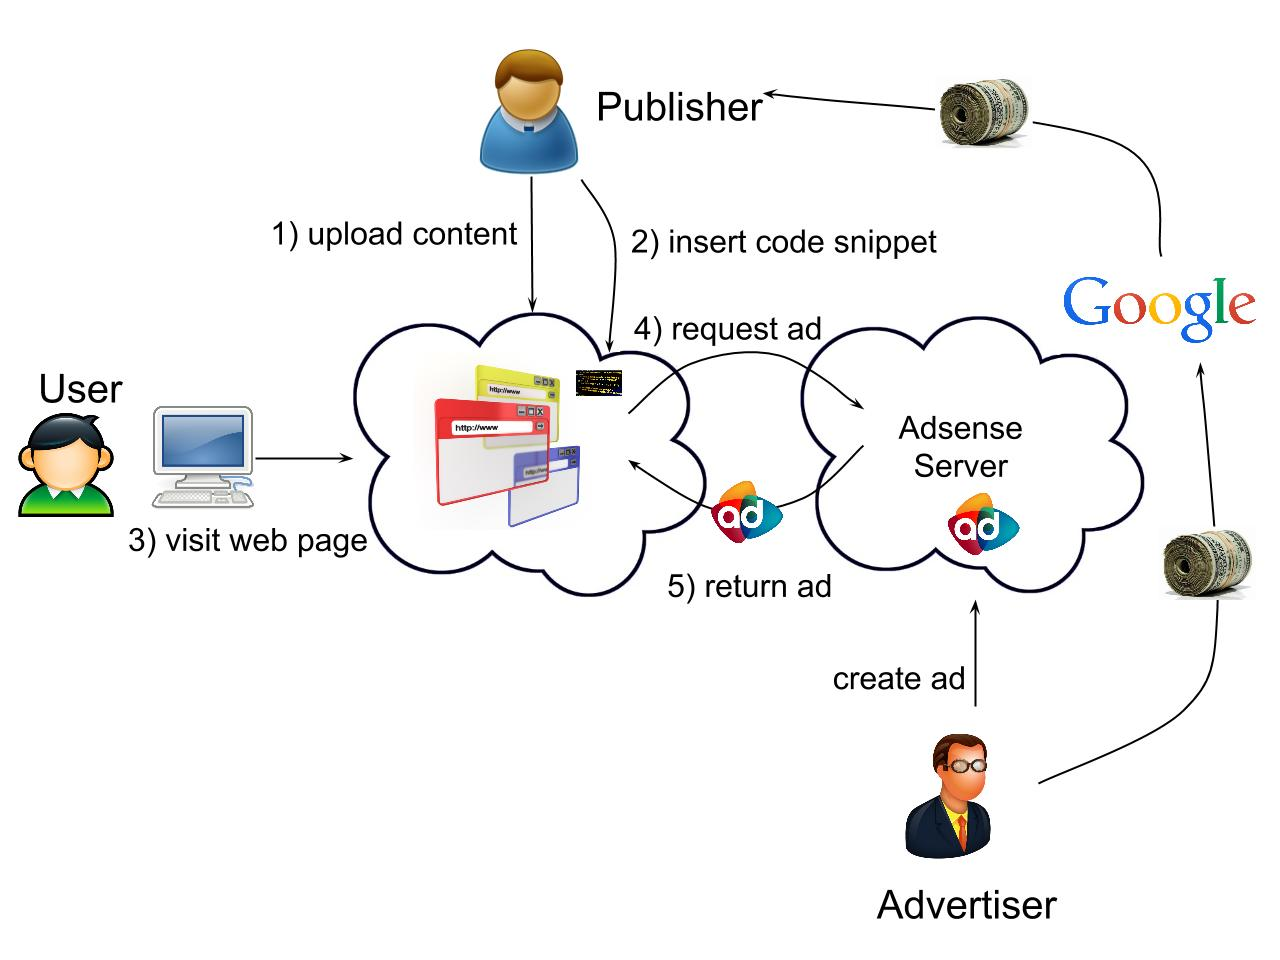
\includegraphics[width=0.4\textwidth]{figures/adsense.jpg}
  \caption{Google Adsense system work flow.}
  \label{fig:adsense}
\end{figure}

\textcolor{red}{ PLEASE ADD SOME DESCRIPTION HERE: To maximize the
  click through rate, the adverstisement keywords need to be more
  semantic relevant as possible.  Also historical data needs to be use
  to predict the potential good keywords to improve the overall click
  through rate. The adsense system will provide a candidate keyword
  lists to advertisers, which can potentially maximize their business
  income.  There are hundrads of millions of advertisements online,
  and huge amount of possible keywords. How to select a good set of
  candidate keywords to publisher is not easy. }
